\section{Experiment}
%\begin{figure}[t]
%	\centering
%	%\fbox{\rule{0pt}{2in} \rule{0.9\linewidth}{0pt}}
%	\includegraphics[width=0.8\linewidth]{experiment.png}
%	
%	\caption{Assessing the Similarity Between Network Activation and Brain Activation.}
%	\label{fig:fig3}
%\end{figure}
%\label{sec:experiment}

\subsection{Benchmarks} \label{sec:Dataset}

All evaluations are completed on CARLA simulator \cite{Dosovitskiy:2017} 0.9.10. 
We evaluate our methods on the NoCrash\cite{codevilla2019exploring} and the LeaderBoard  benchmark.
Each benchmark specified its training towns and weather, where agent is allowed to collect data, and evaluates the agent in new towns and weather.
The NoCrash benchmark considers generalization from Town01, a European town composed of solely one-lane roads and T-junctions, to Town02, a smallker version of Town01 with different textures.
By contrast, the LeaderBoard considers a more difficult generalization task in six maps that cover diverse traffic situations, including freeways, US-style junctions, roundabouts, stop signs, lane changing and merging.
Following the NoCrash benchmark, we test generalization from four training weather types to two new weather types.
But to save computational resources, only two out of the four training weather types are evaluated.
The NoCrash benchmark comes with three levels of traffic density (empty, regular and dense), which defines the number of pedestrians and vehicles in each map.
We focus on the NoCrash-dense and introduce a new level between regular and dense traffic, NoCrash-busy, to avoid congestion that often appears in the dense traffic setting.
For the offline LeaderBoard the traffic density in each map is tuned to be comparable to the busy traffic setting. 


% CILv2
As recent top-performing methods \cite{Hu:2022}, for on-board data collection in CARLA, we use the \emph{teacher} expert driver from \cite{Zhang:2021}, termed as Roach RL since it is based on reinforcement learning and was trained with privileged information. 
Roach RL shows a more realistic and diverse behavior than the default (handcrafted) expert driver in CARLA. 
Note that in real-world experiments we would use different human drivers as experts. 
We use the default settings of \cite{Zhang:2021}, so as in the \emph{student} driver of \cite{Zhang:2021} (RIM) as well as in \cite{Hu:2022} (MILE), the ego-vehicle is the Lincoln 2017 available in CARLA. 
Each of our three forward-facing cameras on-board the ego-vehicle has a resolution of $W\times H=300\times300$ pixels, covering an HFOV of $60^{\circ}$. 
They are placed without overlapping so that they jointly cover an HFOV=$180^{\circ}$ centered in the main axis of the ego-vehicle. 


With such expert driver, ego-vehicle, and on-board cameras, we collect data for increasingly complex experiments. 
First, we collect a dataset from Town01 in CARLA, which is a small town only enabling single-lane driving, {\ie}, lane change maneuvers are not possible. 
% 中午、傍晚、大雨的中午、潮湿的中午
In particular, we collect 15 hours of data at 10 fps ($\sim$540K frames from each camera view), under 4 training weathers, namely, ClearNoon, ClearSunset, HardRainNoon, and WetNoon. 
% 测试:Town02 细雨的傍晚、潮湿的傍晚
In this case, CARLA's Town02 is used for generalization testing under SoftRainSunset and WetSunset weather conditions. 
Second, we collect a dataset from multiple CARLA's towns to include more complex scenarios such as multi-lane driving, entering and exiting highways, passing crossroads, {\etc} In order to keep the same setting as \cite{Hu:2022}, we hold Town05 for testing, and collect 25 hours of data at 10 fps from Town01 to Town06 (5 hours per town; $\sim$900K frames from each camera). 
Training and testing weathers are the same for both Town01 and Town02. 



\subsection{Implementation Details}
To optimize Eq. (\ref{eq:loss}), we use the Adam \cite{Kingma:2015} with an initial learning rate of $10^{-4}$ and weight decay of $0.01$. 
We train for 80 epochs on 1 NVIDIA A100 GPUs, with a batch size of 120. 
The learning rate decays by half at epochs 30, 50, and 65. 

% 其他
%During the experiment, we randomly selected start and target positions, and computed the route using A* algorithm. 
%Subsequently, we executed $\pi_{\theta_{k}}$ in the CARLA~\cite{Dosovitskiy17} environment to gather trajectory data and synchronized brain activation record.
%We employed a specific reward scheme and imposed additional penalties for large steering changes to prevent oscillatory maneuvers. 
%After training the network, we compared the similarity between the network activations and those observed in the human brain. 
%As depicted in Fig.~\ref{fig:fig3}, we contrasted the similarity between the test participant and the brain-inspired network in processing the same event.


% 驾驶评估的3个不同数据集
\subsection{Driving Evaluation}
\label{sec:Metrics}
The performance of the BID agent is constrained by the performance of the expert it is imitating. 
When the expert performs poorly, the agent that mimics the expert will also exhibit poor performance. 
The BID model is designed in strict accordance with the human brain's visual information processing process, both structurally and functionally. 
When optimized, the model's output results are very close to those of the expert in terms of evaluating the similarity.


We follow the \emph{NoCrash} benchmark~\cite{Codevilla:2019} and the offline CARLA leaderboard benchmark~\cite{Zhang:2021,Hu:2022} for experiments on small single-lane towns (Sec.~\ref{sec:small_town_results}) and multiple towns (Sec.~ \ref{sec:multi_towns_result}), respectively.


\subsubsection{NoCrash Metrics.}\label{nocrash_metrics}
It consists of 3 tasks with increasing levels of difficulty: \emph{Empty}, \emph{Regular}, and \emph{Dense}, according to the number of dynamic objects in the scene ({\ie}, pedestrians and vehicles). 
In Town 2, the numbers of dynamic objects are specified as:
\begin{itemize}
	\item \emph{Empty}: 0 pedestrian and 0 vehicle;
	\item \emph{Regular}: 50 pedestrians and 15 vehicles;
	\item \emph{Dense}: 150 pedestrians and 70 vehicles
\end{itemize}
% 默认的配置会导致拥堵死锁
In the \emph{Dense} case, the default traffic density set in NoCrash always leads to congestion deadlocks at intersections \cite{Zhang:2021}. 
Thus, we follow the \emph{Busy} case redefined in \cite{Zhang:2021}, decreasing the number of pedestrians from 150 to 70. 
Each task corresponds to 25 goal-directed episodes under 2 new kinds of weather.
The episode will be terminated and counted as a failure once a collision occurs. 
For the other infractions, the driving score will be deduced according to the penalty rule in NoCrash. 


% 度量标准的说明
The main metric to compare driving models is the success rate (\emph{SR}), which is the percentage of episodes successfully completed. 
% 严格的成功率
For a fine-grained comparison, in addition, we provide the strict success rate (\emph{S.SR}). 
% traffic infraction:交通违法行为
It reflects the percentage of successful episodes under zero tolerance for any traffic infraction, such as failing to stop at a red traffic light, route deviation, {\etc}. 
% T.L:在红灯时不停的次数
As a complement, we also include additional infraction metrics: \emph{T.L} is the number of times not stopping at a red traffic light; 
% 和其他车辆碰撞的次数
\emph{C.V} is the number of collisions with other vehicles; 
% R.Dev:当高层命令没有很好地执行,路线偏差的次数
\emph{R.Dev} is the number of route deviations, {\ie}, when the high-level command is not well-executed; 
% O.L:考虑了自主车辆驶出车道的情况(例如,在对面车道或人行道上)
\emph{O.L} accounts for the ego-vehicle driving out-of-lane ({\eg}, in the opposite lane or in the sidewalk); 
% C.L:与城镇布局发生碰撞的次数
\emph{C.L} is the number of collisions with the town layout. 
All infraction values are normalized per driven kilometer.


\subsubsection{Offline Leaderboard Metrics.}\label{lb_metrics}
To align our evaluation with leaderboard\cite{Hu:2022}, we use the offline CARLA's Leaderboard metrics for multiple towns. 
% Avg.DS 平均驾驶分数、平均路线完成
The most important metrics are the average driving score (\emph{Avg.DS}) and the average route completion (\emph{Avg.RC}). 
\emph{Avg.DS} is based on penalizing driving performance according to the terms defined in CARLA's Leaderboard, 
% Avg.RC:自车辆能够行驶至目标的平均距离。
while \emph{Avg.RC} is the average distance towards the goal that the ego-vehicle is able to travel.


% 高层导航命令
\subsubsection{High-level Navigation Commands} 
As in CILRS \cite{Codevilla:2019}, at training time we use simple navigation commands such as \emph{continue} in the lane, or \emph{go-straight/turn-left/turn-right} next time an intersection is reached. 
However, in complex towns, after crossing an intersection in any direction, we may legally enter any of the multiple lanes. 
Thus, since this can be known by the global navigation system, when the ego-vehicle enters a lane out of the pre-planned global trajectory, a corrective command is forced, like \emph{move-to-left-lane} or  \emph{move-to-right-lane} as soon as possible. 
This corrective mechanism is used only at testing time. 
Figure~\ref{fig:command_ambiguous} provides an example.

\begin{figure}[t]
	\centering
	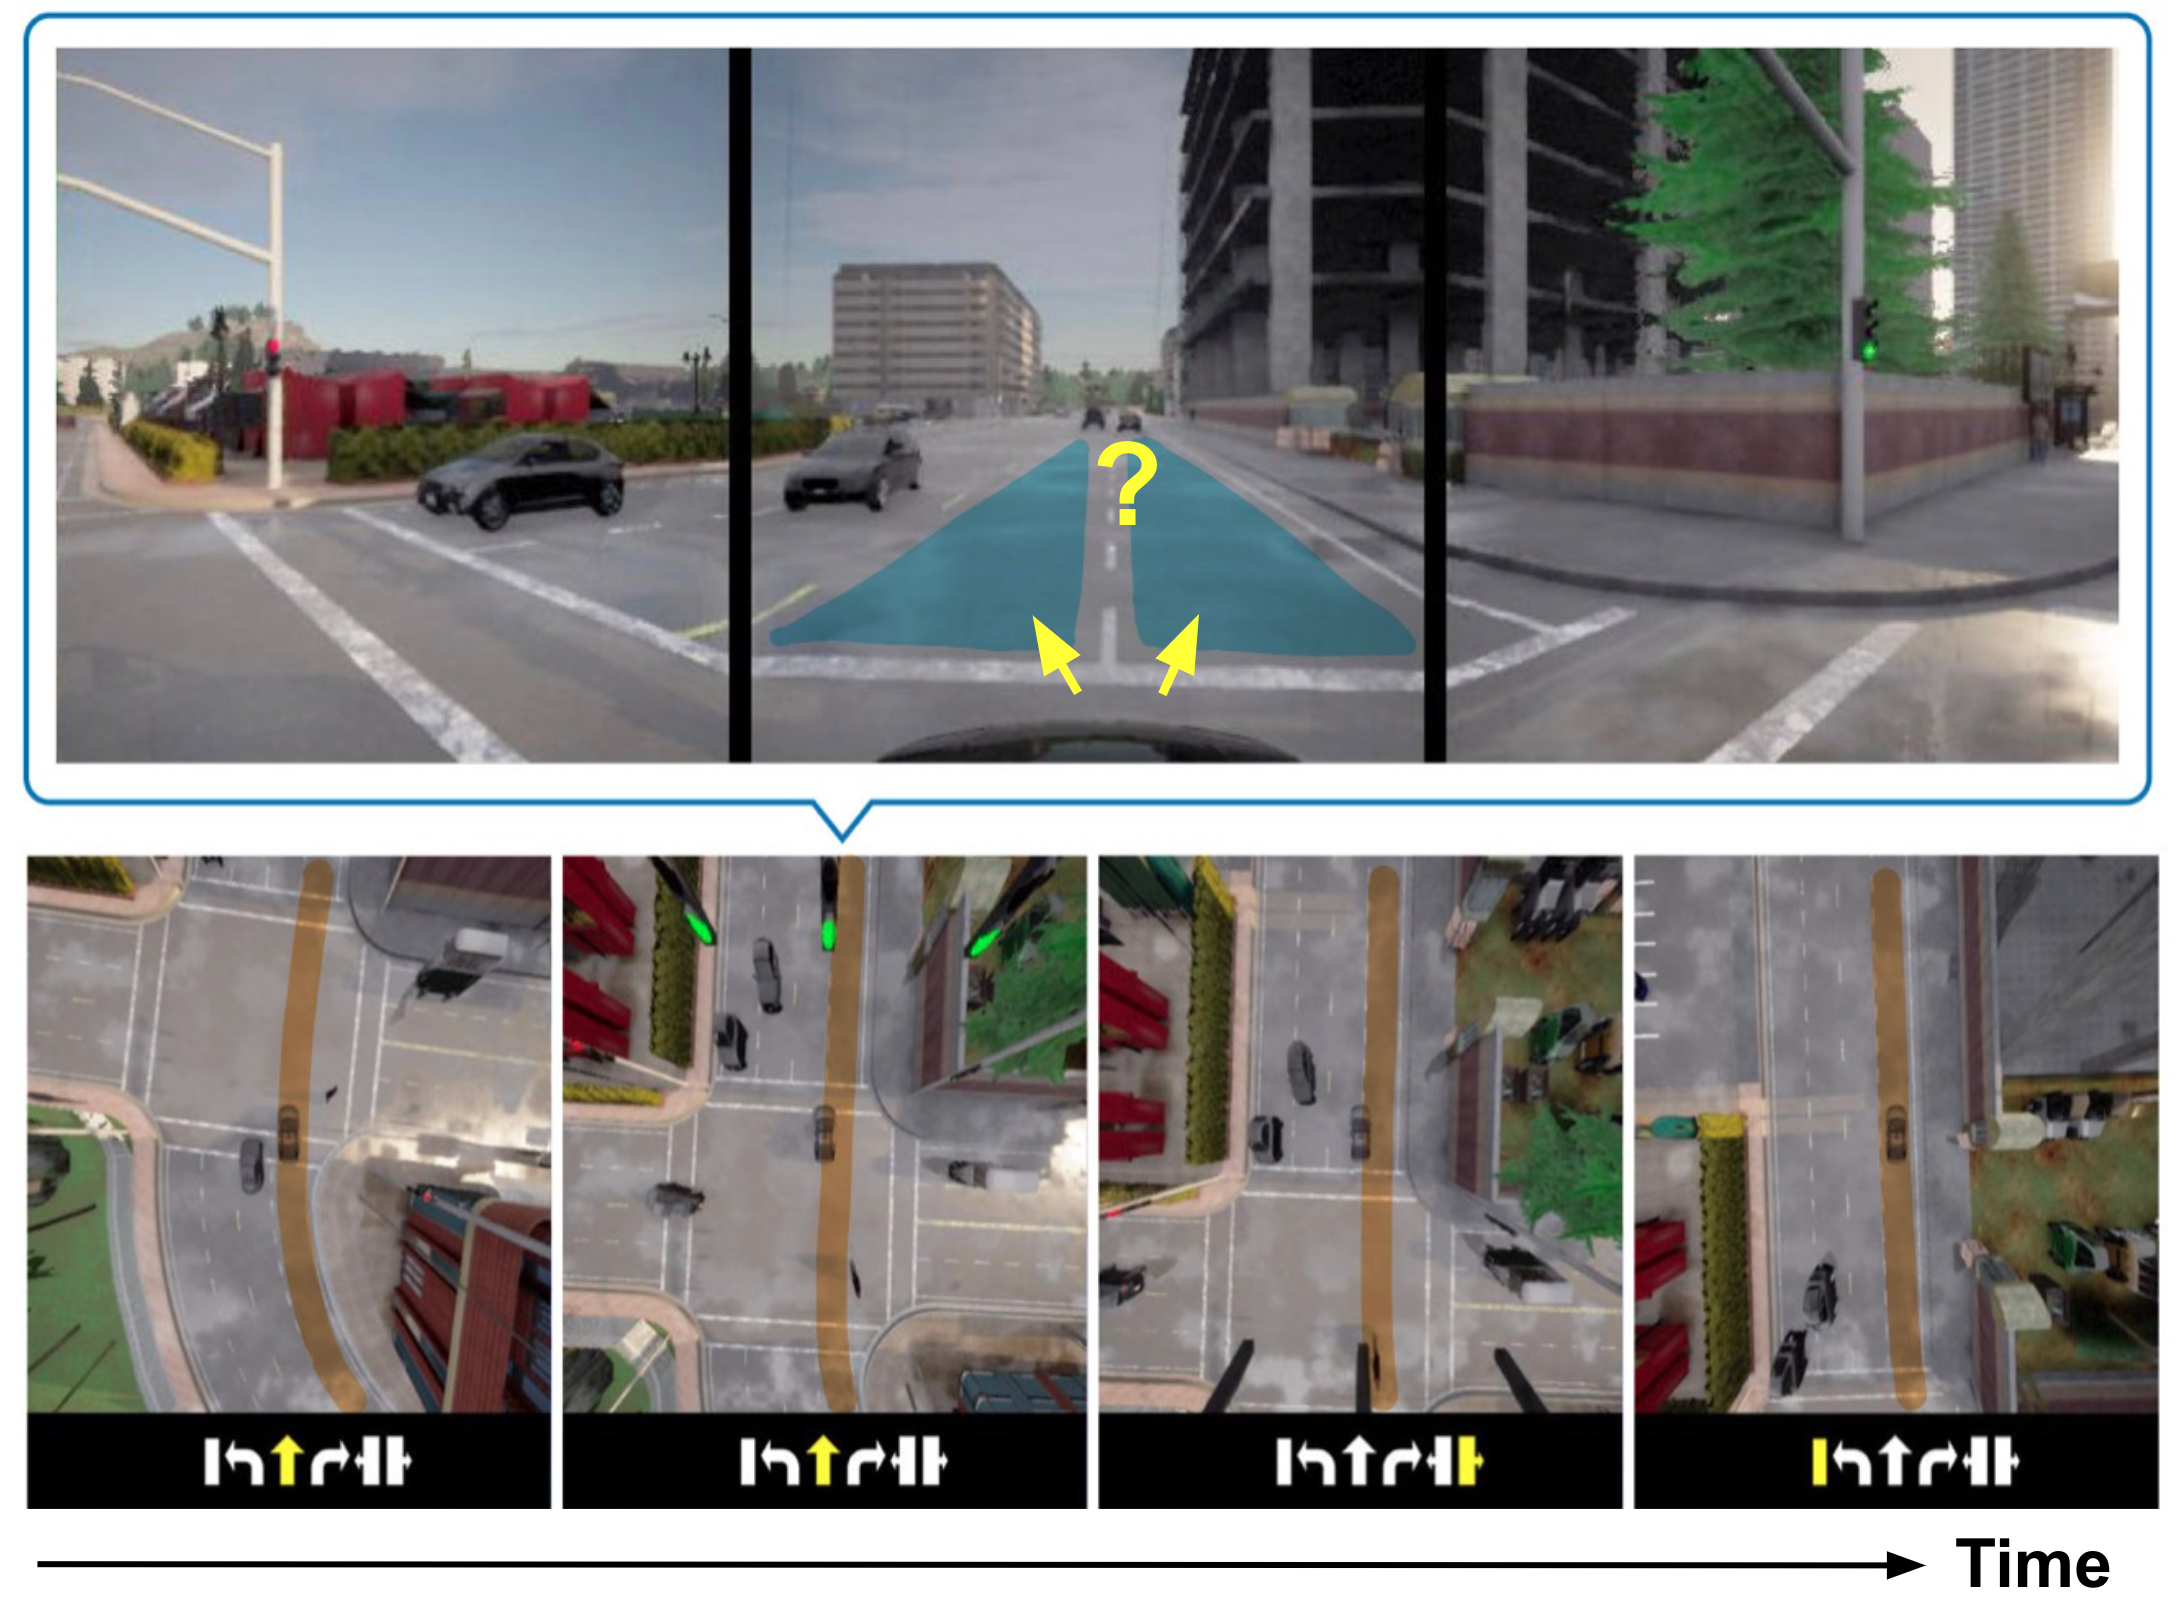
\includegraphics[width=1.0\linewidth]{fig/cmd_ambiguous.png}
	\caption{Top: when the ego-vehicle is entering a new road segment from an intersection, the \emph{go-straight} navigation command is ambiguous. 
	The ego-vehicle can legally move to any of the highlighted lanes. 
	Bottom: four aerial views at different times with the pre-planned global trajectory shown in \textbf{\textcolor{orange}{orange}}. 
	They illustrate how the high-level navigation command changes to \emph{move-to-right-lane}, to inform how to get back to the desired trajectory.}
	\label{fig:command_ambiguous}
\end{figure}


\begin{table*}
	\centering
	\resizebox{0.95\linewidth}{!}{
		\begin{tabular}{@{}lccc|ccc|ccc@{}}
			\toprule
			& \multicolumn{3}{c}{Empty} & \multicolumn{3}{c}{Regular} & \multicolumn{3}{c}{Busy}  \\
			
			& \textbf{$\uparrow$ SR(\%)} & \textbf{$\uparrow$ S.SR(\%)} & $\downarrow$ T.L  & \textbf{$\uparrow$ SR(\%)} & \textbf{$\uparrow$ S.SR(\%)} & $\downarrow$ T.L & \textbf{$\uparrow$ SR(\%)} & \textbf{$\uparrow$ S.SR(\%)} & $\downarrow$ C.V \\
			\midrule
			
			RIM\cite{Zhang:2021}  & $100\pm0.0$ & $85\pm1.2$ & $66\pm5.0$ & $97\pm2.3$ & $86\pm7.2$ & $66\pm54$ & $81\pm5.0$& $68\pm7.2$ & $63\pm52.7$\\
			CIL++ & $100\pm0.0$ & $100\pm0.0$ & $0\pm0.0$  & $99\pm2.3$ & $97\pm3.1$ & $7\pm7.9$ & $83\pm7.6$ & $77\pm7.6$ & $45\pm21.5$ \\
			BID & $100\pm0.0$ & $100\pm0.0$ & $0\pm0.0$  & $99\pm2.3$ & $97\pm3.1$ & $7\pm7.9$ & $83\pm7.6$ & $77\pm7.6$ & $45\pm21.5$ \\
			\midrule
			Expert & $100\pm0.0$ & $100\pm0.0$ & $0\pm0.0$ & $100\pm0.0$ & $97\pm0.0$ & $13\pm4.6$ & $84\pm2.0$ & $82\pm2.0$ & $37\pm14.1$ \\
			\bottomrule 
		\end{tabular}
	}
	\caption{Town02 NoCrash results.
		RIM stands for Roach IL and the Expert is Roach RL~\cite{Zhang:2021}. 
		All models are tested on CARLA 0.9.13. 
		Mean and standard deviations are computed using three runs with different seeds. 
		For $\uparrow$, the higher the better, while for $\downarrow$ is the opposite.}
	\label{tab:T2_NC_results}
\end{table*}


\begin{table*}
	\centering
	\resizebox{0.95\linewidth}{!}{
		\begin{tabular}{@{}lcccccccccccccccc@{}}
			\toprule
			&  \textbf{$\uparrow$ SR(\%)} &  \textbf{$\uparrow$ S.SR(\%)} &  \textbf{$\uparrow$ Avg.RC(\%)} &  \textbf{$\uparrow$ Avg.DS}  
			& $\downarrow$ C.L & $\downarrow$ T.L & $\downarrow$ O.L & $\downarrow$ R.Dev 
			\\
			\midrule
			HFOV $100^{\circ}$ & $52$ & $40$ & $83$ & $69.1$ 
			&$428.6$& $19.6$ & $ 339.6$ & $10.7$ 
			\\
			HFOV $180^{\circ}$ & $100$ & $98$ & $100$ & $99.2$ 
			&$7.3$& $0.0$ & $0.0$ & $0.0$ 
			\\
			\midrule
			Expert & $100$ & $100$ & $100$ & $100.0$ 
			& $0.0$ & $0.0$ & $0.0$ & $0.0$ 
			\\
			\bottomrule 
		\end{tabular}
	}
	% 视场角(Field of View, FOV),包括水平视场角(HFOV)、垂直视场角(VFOV)和对角视场角(DFOV)
	\caption{Impact of sensor suite HFOV in the NoCrash Regular case.
		For HFOV=$100^{\circ}$ we use a single camera with a resolution of $W\times H=600\times170$ pixels, while for HFOV=$180^{\circ}$ we use the multi-view setting detailed in the main text.}
	\label{tab:FOVresults}
\end{table*}

\begin{table*}
	\centering
	\resizebox{0.95\linewidth}{!}{
		\begin{tabular}{@{}lccccccccccccccccccccc@{}}
			\toprule
			%   & SR(\%) 
			%   & S.SR(\%) 
			& \textbf{$\uparrow$ Avg.RC(\%)} & \textbf{$\uparrow$ Avg.DS }
			& $\downarrow$ C.V & $\downarrow$ C.L & $\downarrow$ T.L & $\downarrow$ O.L & $\downarrow$ R.Dev 
			\\
			\midrule
			RIM\cite{Zhang:2021}  & $92\pm3.1$ & $51\pm7.9$ 
			& $7.5\pm1.3$ & $4.3\pm1.6$ & $26.0\pm8.9$ & $5.4\pm2.7$ & $3.0\pm3.2$ & \\
			MILE~\cite{Hu:2022}
			& $98\pm2.2$ & $73\pm2.9$ 
			& $6.0\pm3.7$ & $0.0\pm0.0$ & $3.6\pm3.8$ & $3.5\pm1.5$ & $0.0\pm0.0$ \\   
			CIL++ 
			& $98\pm1.7$ & $68\pm2.7$ 
			& $6.0\pm0.5$ & $3.8\pm0.7$ & $5.8\pm5.1$ & $6.1\pm2.2$ & $9.4\pm3.6$ \\
			BID 
			& $98\pm1.7$ & $68\pm2.7$ 
			& $6.0\pm0.5$ & $3.8\pm0.7$ & $5.8\pm5.1$ & $6.1\pm2.2$ & $9.4\pm3.6$ \\
			\midrule
			Expert 
			& $99\pm0.8$ & $89\pm1.7$ 
			& $3.2\pm1.1$ & $0.0\pm0.0$ & $1.3\pm0.4$ & $0.0\pm0.0$ & $0.0\pm0.0$ \\
			\bottomrule 
		\end{tabular}
	}
	\caption{Town05 results according to CARLA's offline metrics. All models are tested on CARLA 0.9.13. 
		Mean and standard deviations are computed using three runs with different seeds. 
		For $\uparrow$, the higher the better; for $\downarrow$, the opposite.}
	\label{tab:T5_results}
\end{table*}


\begin{table}
	\centering
	\begin{tabular}{@{}lccccc@{}}
		\toprule
		& $\uparrow$ SR(\%) & $\uparrow$ S.SR(\%) & $\uparrow$ Avg.RC(\%) & $\uparrow$ Avg.DS  \\
		\midrule
		LF.A & $72$ & $62$ & $86$ & $78.1$  \\
		LF.C & $76$ & $66$ & $88$ & $80.6$  \\
		Token & $88$ & $80$ & $93$ & $88.4$  \\
		CIL++ & $88$ & $84$ & $93$ & $88.8$  \\ 
		\bottomrule 
	\end{tabular}
	\caption{Results of different data input fusion approaches for NoCrash Busy scenarios.}
	\label{tab:ablation_study_inputfusion}
\end{table}

\begin{table}
	\centering
	\begin{tabular}{@{}lcccccccccccccccc@{}}
		\toprule
		& $\uparrow$ SR(\%) & $\uparrow$ S.SR(\%) & $\uparrow$ Avg.RC(\%) & $\uparrow$ Avg.DS  \\
		\midrule
		GAP & $64$ & $46$ & $87$ & $75.1$  \\
		VS & $70$ & $62$ & $89$ & $78.6$  \\
		CIL++ & $88$ & $84$ & $93$ & $88.8$  \\ 
		\bottomrule
	\end{tabular}
	\caption{Results of different multi-view fusion approaches for NoCrash Busy scenarios.}
	\label{tab:ablation_study_sa}
\end{table}


\subsection{Experimental Results}
\label{sec:Results}
% 基于模型的模仿学习
We compare BID with two SOTA vision-based EtE-AD models, namely, the Roach IL model (here RIM) \cite{Zhang:2021}, MILE \cite{Hu:2022} and CIL++. 
Notice that although CIL++ uses the data generated by the Roach RL model, essentially training a CIL++ model does not require human-labeled sensor data. 
In our case, the Roach RL plays the role of a human driver at data acquisition time. 
In contrast, training a RIM model requires teaching from the Roach RL expert who was trained with privileged information, while MILE is trained with semantic BeV as supervision.


\subsubsection{Small Single-lane Towns} \label{sec:small_town_results}
We first use CARLA's Town01 and Town02 along with the NoCrash metrics (Sec.~\ref{nocrash_metrics}) for initial experiments. 
Town01 is used for training and Town02 for testing (Sec.~\ref{sec:Dataset}). 
MILE only provides a model trained on CARLA's multiple towns, but there is no model trained only on Town01, while RIM has versions trained on Town01 and multiple towns. 
Thus, for a fair comparison, we only use RIM's single-town trained model. 
We show in Table~\ref{tab:T2_NC_results} SR and S.SR for the considered traffic densities (Empty, Regular, Busy). 
In order to have a more focused evaluation, we show T.L only for the Empty and Regular cases, while C.V is shown only for the Busy case. 
Note that scenarios with no or few dynamic obstacles can better show the ego-vehicle reaction to red traffic lights, while collisions are better evaluated in scenarios with more dynamic objects. 


In general, CIL++ achieves the best results in all the tasks. 
In the Empty case, CIL++ clearly outperforms RIM in avoiding traffic light infractions, which also contributes to a better S.SR. We reach the same conclusion in the Regular case. 
In the Busy case, CIL++ reaches almost the expert's performance, again, being clearly better than RIM for S.SR and producing fewer collisions with vehicles. 
For the expert, the failure cases in Busy scenarios are due to traffic deadlocks, which lead to a timeout in route completion. 
Thus, its performance still can be considered as a proper upper bound. 


Traffic lights tend to be on sidewalks, so detecting them from a close distance requires a sensor setting with a proper HFOV. 
Otherwise, causal confusion can appear. 
We think that the poor performance of RIM on the T.L metric is due to a narrow HFOV as illustrated in Fig.~\ref{fig:causalconfusion}.  
To confirm this hypothesis, we conduct experiments using two HFOV settings for CIL++, 100 and 180. 
As seen in Table~\ref{tab:FOVresults}, we note that the number of infractions (T.L, C.L, O.L, R.Dev) increase when we use a lower HFOV=$100^\circ$ compared to HFOV=$180^\circ$. 
For HFOV=$100^\circ$, we have observed that the track of the road shoulder is easily out-of-observation at intersections, leading to more O.L, C.L, and R.Dev. 
For HFOV=$180^{\circ}$, the ego-vehicle can better perform the right driving maneuver, thanks to having the road shoulder as a reference.


\begin{figure}
	\centering
	\begin{subfigure}[b]{\linewidth}
		\centering
		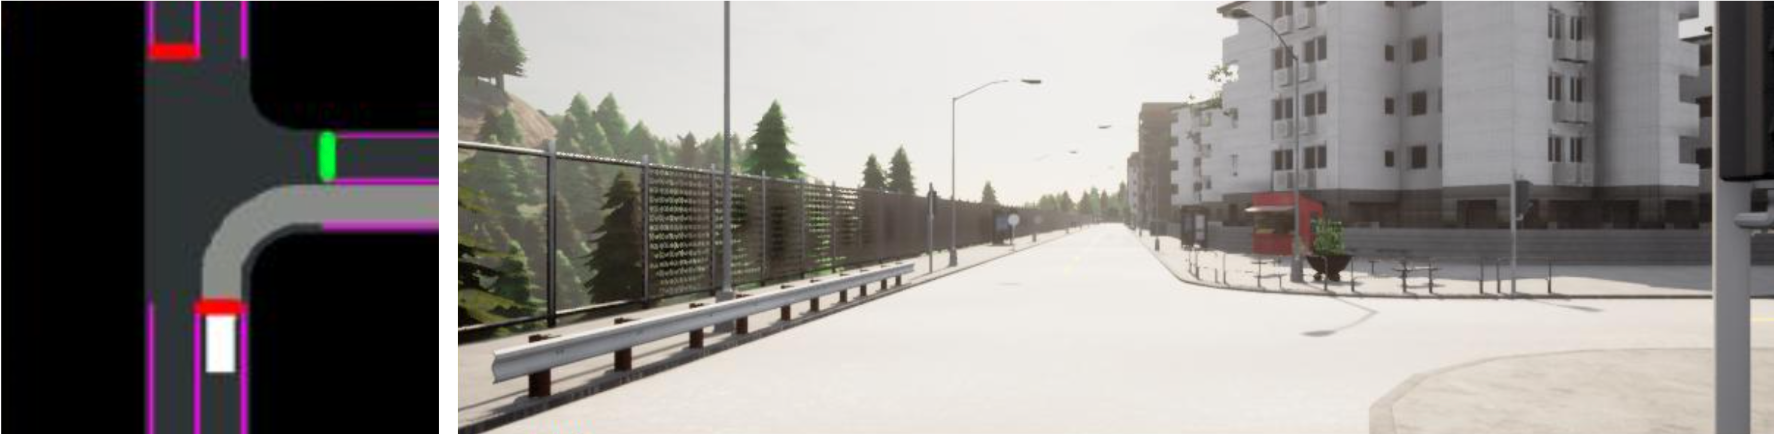
\includegraphics[width=\textwidth]{fig/TLCausalConfusionA.png}
		\caption{Roach RL \cite{Zhang:2021}: using semantic BeV as input during training time}
		\label{fig:TLCausualConfusionB}
	\end{subfigure}
	\hfill
	\begin{subfigure}[b]{\linewidth}
		\centering
		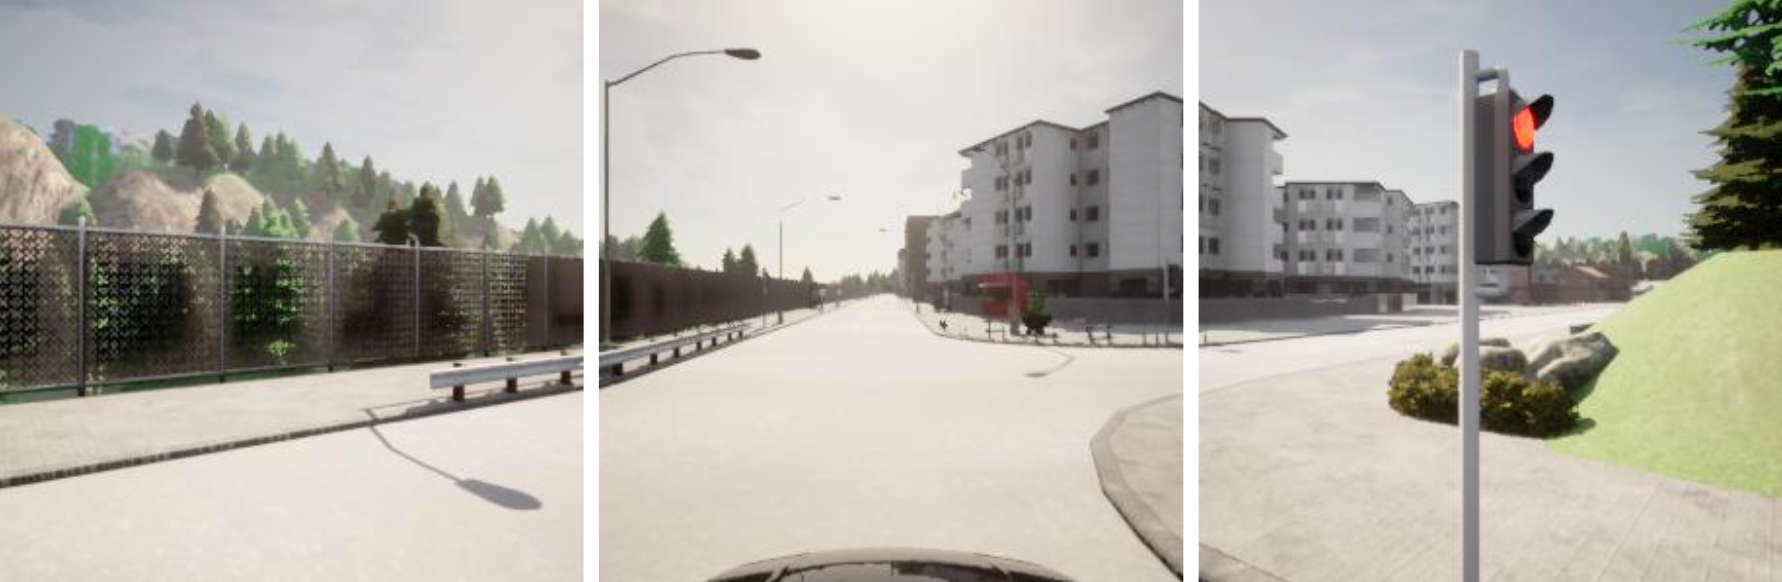
\includegraphics[width=\textwidth]{fig/TLCausalConfusionB.png}
		\caption{CIL++: only images from three views as input}
		\label{fig:TLCausualConfusionA}
	\end{subfigure}
	%   \includegraphics[width=1.0\linewidth]{images/TLcausalConfusion.png}
	\caption{Top Left: The expert we use for data collection is the teacher agent Roach RL \cite{Zhang:2021}, which has access to semantic BeVs. 
		Note that, in simulation, this expert plays the role of a human driver in the real world, who would drive to collect on-board data. 
		Top Right: Using an insufficient FOV, the red traffic light is not observable in the image when the expert stops close to it, which may cause causal confusion when applying imitation learning to train the student agent RIM. 
		Bottom: CIL++ avoids this causal confusion by using a larger HFOV based on three complementary images (from different cameras). More specifically, RIM uses HFOV=$100^{\circ}$, while CIL++ uses HFOV=$180^{\circ}$.}
	\label{fig:causalconfusion}
\end{figure}


\subsubsection{Multi-town Generalization}\label{sec:multi_towns_result}
In this section, we assess the performance of CIL++ in much more complex scenarios, as provided by CARLA's multiple towns. 
As mentioned in Sec.~\ref{sec:Dataset}, for a fair comparison, we align the training and testing settings with MILE~\cite{Hu:2022}, using CARLA's offline Leaderboard metrics (Sec.~\ref{lb_metrics}).
The results for all models trained on multi-town data are shown in Table~\ref{tab:T5_results}. 
RIM shows the worst performance among the three models, incurring more infractions, thus obtaining a significantly lower Avg.DS. 
CIL++ achieves 98\% Avg.RC, which is on par with MILE. 
In terms of Avg.DS, MILE remains the best scoring, yielding a 73\% while CIL++ achieves a 68\%. 
We observe that this is because MILE seldom drives outside the pre-planned lane, given the route map as input. 
On the contrary, CIL++ lacks the explicit use of this route map since it only receives high-level navigation commands. 


% 速度、目标?
%\subsubsection{Ablation Study}
%\label{sec:Ablation Study}
%To inspect the impact of some components of CIL++, we provide an ablation study. 
%Specifically, we are interested in the fusions of input data and multi-view. 
%
%\paragraph{Input Data Fusion}
%EtE-AD models require not only sensor data but also signal information, like the ego-vehicle speed and a high-level navigation command. 
%It is interesting to study how to properly fuse these inputs. 
%To compare, we implement several types of input data fusion in Table~\ref{tab:ablation_study_inputfusion}: adding, concatenation, and tokenization. 
%In the first, the speed and command features are simply added to the image features. 
%This addition could be done either before (the default operation in CIL++) or after the Transformer Encoder block. 
%We name the latter as late fusion adding (LF.A). 
%Another common data fusion method is concatenation, which firstly stacks all the features and takes an extra join FC layer to fuse them, which we term as late fusion concatenation (LF.C). 
%Since the transformer model uses a self-attention mechanism to fuse features between tokens, we can tokenize the speed and navigation command features and feed them into the transformer block along with the image features. 
%We term this approach as Token. 
%Our results suggest that there is no obvious difference between tokenization and early adding fusion. 
%These two approaches show better results than the late fusion.
%
%
%\paragraph{Multi-view Fusion}
%CIL++ uses attention layers to fuse multi-view information. 
%To understand their contribution, we remove the transformer block and simply use the ResNet34 which retains the average pooling and an FC layer for embedding each image view. 
%The embedding outputs are then stacked and fed to the FC join layers for fusion. 
%We term this approach as view stacking (VS) in Table~\ref{tab:ablation_study_sa}. 
%The speed and command features are added to the joint embedding before feeding into the action prediction MLP. 
%We see that without the self-attention layers, the SR drops from 88\% to 70\%. 
%We think this is because the average pooling layer causes a loss of spatial information, while this information is very important for actual driving. 
%The agent should take different actions according to the location of dynamic obstacles. 
%We also use a transformer block to process the output of the ResNet average pooling layer (GAP), instead of using the flattened feature map from the last convolutional layer of ResNet34. 
%The results drop significantly, {\eg}, and the SR goes from 88\% to 64\%.


\begin{figure}[t]
	\begin{center}
		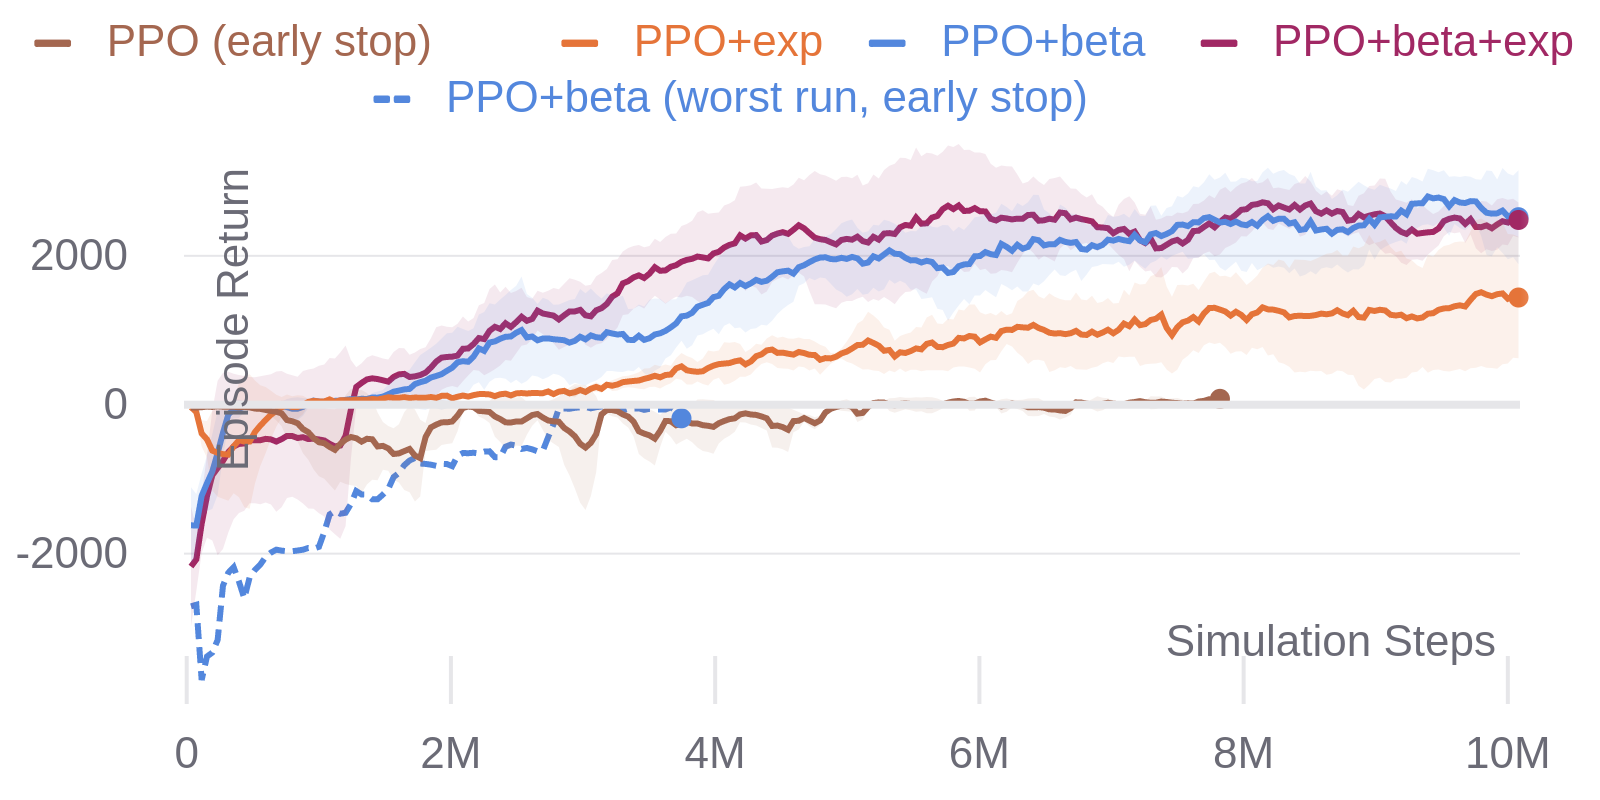
\includegraphics[width=\linewidth]{img/rl.png}
	\end{center}
	\vspace{-4ex}
	\caption{\textbf{Learning curves of RL experts }
		trained in CARLA Town 1-6.
		Solid lines show the mean and shaded areas show the standard deviation of episode returns across 3 seeds.
		The dashed line shows an outlier run that collapsed.}
	\vspace{-2ex}
	\label{fig:rl}
\end{figure}


\subsection{Performance of Experts}

%\textbf{\textsf{Sample Efficiency:}}
%To improve the sample efficiency of PPO, we propose to use BEV instead of camera images, Beta instead of Gaussian distributions, and the exploration loss in addition to the entropy loss.
%Since the benefit of using a BEV representation is obvious, here we only ablate the Beta distribution and the exploration loss.
%As shown in Fig.~\ref{fig:rl}, the baseline PPO with Gaussian distribution and entropy loss is trapped in a local minimum where staying still is the most rewarding strategy.
%Leveraging the exploration loss, PPO+exp can be successfully trained despite relatively high variance and low sample efficiency.
%The Beta distribution helps substantially, but without the exploration loss the training still collapsed in some cases due to insufficient exploration (cf. dashed blue line in Fig.~\ref{fig:rl}).
%Our Roach (PPO+beta+exp) uses both Beta distribution and exploration loss to ensure stable and sample efficient training.
%The training takes around 1.7M steps in each of the six CARLA servers, this accounts for 10M steps in total, which takes roughly a week on an AWS EC2 g4dn.4xlarge or 4 days on a 2080 Ti machine with 12 cores.



\subsubsection{Driving Performance}

Table~\ref{table:expert_performance} compares different experts on the NoCrash-dense and on all 76 LeaderBoard routes under dynamic weather with busy traffic.
Our Autopilot is a strong baseline expert that achieves a higher success rate than the Autopilot used in LBC and DA-RB.
We evaluate three RL experts - 
(1) Roach, the proposed RL coach using Beta distribution and exploration prior.
(2) PPO+beta, the RL coach trained without using the exploration prior. 
(3) PPO+exp, the RL coach trained without using the Beta distribution.
In general, our RL experts achieve comparable success rates and higher driving scores than Autopilots because RL experts handle traffic lights in a better way (cf. Table~\ref{table:infraction}).
The two Autopilots often run red lights because they drive over-conservatively and wait too long at the junction, thus missing the green light.
Among RL experts, PPO+beta and Roach, the two RL experts using a Beta distribution, achieve the best performance, while the difference between both is not significant. PPO+exp performs slightly worse, but it still achieves better driving scores than our Autopilot. 


\begin{table}
	\setlength{\tabcolsep}{2.32pt}
	\centering
	\begin{tabular}{lccccc}
		\toprule
		Suc. Rate \% $\uparrow$
		& NCd-tt & NCd-tn  & NCd-nt & NCd-nn & LB-all  \\ 
		\cmidrule(lr){1-1}\cmidrule(lr){2-6}
		PPO+exp & $86 \pm 6$ & $86 \pm 6$ & $79 \pm 6$ & $77 \pm 5$ & $67\pm3$  \\
		PPO+beta & $\mathbf{95} \pm 3$ & $\mathbf{95} \pm 3$ & $83 \pm 5$ & $\mathbf{87} \pm 6$ & $72 \pm 5$  \\
		Roach & $91 \pm 4$ & $90 \pm 7$ & $\mathbf{83} \pm 3$ & $83 \pm 3$ & $72 \pm 6$  \\
		\cmidrule(lr){1-1}\cmidrule(lr){2-6}
		AP (ours) & 
		$\mathbf{95} \pm 3$ & $\mathbf{95} \pm 3$ & $83 \pm 5$ & $81 \pm 2$ & $\mathbf{75} \pm 8$ \\
		AP-lbc \cite{chen2020learning}
		& $86 \pm 3$ & $83 \pm 6$ & $60 \pm 3$ & $59 \pm 8$ & N/A \\
		AP-darb \cite{prakash2020exploring}
		& $71 \pm 4$ & $72 \pm 3$ & $41 \pm 2$ & $43 \pm 2$ & N/A \\
		% \bottomrule
		\toprule
		Dri. Score \% $\uparrow$
		& NCd-tt & NCd-tn  & NCd-nt & NCd-nn & LB-all  \\ 
		\cmidrule(lr){1-1}\cmidrule(lr){2-6}
		PPO+exp & $92 \pm 2$ & $92 \pm 2$ & $88 \pm 3$ & $86 \pm 1$ & $ 83\pm0$  \\
		PPO+beta & $\mathbf{98} \pm 2$ & $\mathbf{98} \pm 2$ & $90 \pm 3$ & $\mathbf{92} \pm 2$ & $\mathbf{86} \pm 2$  \\
		Roach & $95 \pm 2$ & $95 \pm 3$ & $\mathbf{91} \pm 3$ & $90 \pm 2$ & $85 \pm 3$  \\
		% Roach
		% & $93 \pm 1$ & $91 \pm 1$ & $91 \pm 4$ & $91 \pm 4$
		% & $79 \pm 1$ \\
		\cmidrule(lr){1-1}\cmidrule(lr){2-6}
		AP (ours)
		& $86 \pm 2$ & $86 \pm 2$ & $70 \pm 2$ & $70 \pm 1$
		& $78 \pm 3$ \\
		\bottomrule
	\end{tabular}
	\vspace{-1ex}
	\caption{\textbf{Success rate and driving score of experts.} Mean and standard deviation over 3 evaluation seeds. 
	NCd: NoCrash-dense. 
	tt: train town \& weather. 
	tn: train town \& new weather. 
	nt: new town \& train weather. 
	nn: new town \& weather. 
	LB-all: all 76 routes of LeaderBoard with dynamic weather. 
	AP: CARLA Autopilot. 
	For RL experts the best checkpoint among all training seeds and runs is used.}
	\label{table:expert_performance}
	\vspace{-2ex}
\end{table}



\subsection{Performance of IL Agents}

The performance of an IL agent is limited by the performance of the expert it is imitating.
If the expert performs poorly, it is not sensible to compare IL agents imitating that expert.
As shown in Table~\ref{table:expert_performance}, this issue is evident in the NoCrash new town with dense traffic, where Autopilots do not perform well. 
To ensure a high performance upper-bound and hence a fair comparison, we conduct ablation studies (Fig.~\ref{fig:score_eu_lb_tt_tn} and Table~\ref{table:infraction}) under the busy traffic setting such that our Autopilot can achieve a driving score of 80\% and a success rate of 90\%. 
In order to compare with the state-of-the-art, the best model from the ablation studies is still evaluated on NoCrash with dense traffic in Table~\ref{table:sucess_rate_nc_dense}.


The input measurement vector $\mathbf{m}_\text{IL}$ is different for the NoCrash and for the LeaderBoard. 
For NoCrash, $\mathbf{m}_\text{IL}$ is just the speed.
For the LeaderBoard, $\mathbf{m}_\text{IL}$ contains additionally a 2D vector pointing to the next desired waypoint.
This vector is computed from noisy GPS measurements and the desired route is specified as sparse GPS locations.
The LeaderBoard instruction suggests that it is used to disambiguate situations where the semantics of left and right are not clear due to the complexity of the considered map.
\begin{figure*}[t]
	\centering
	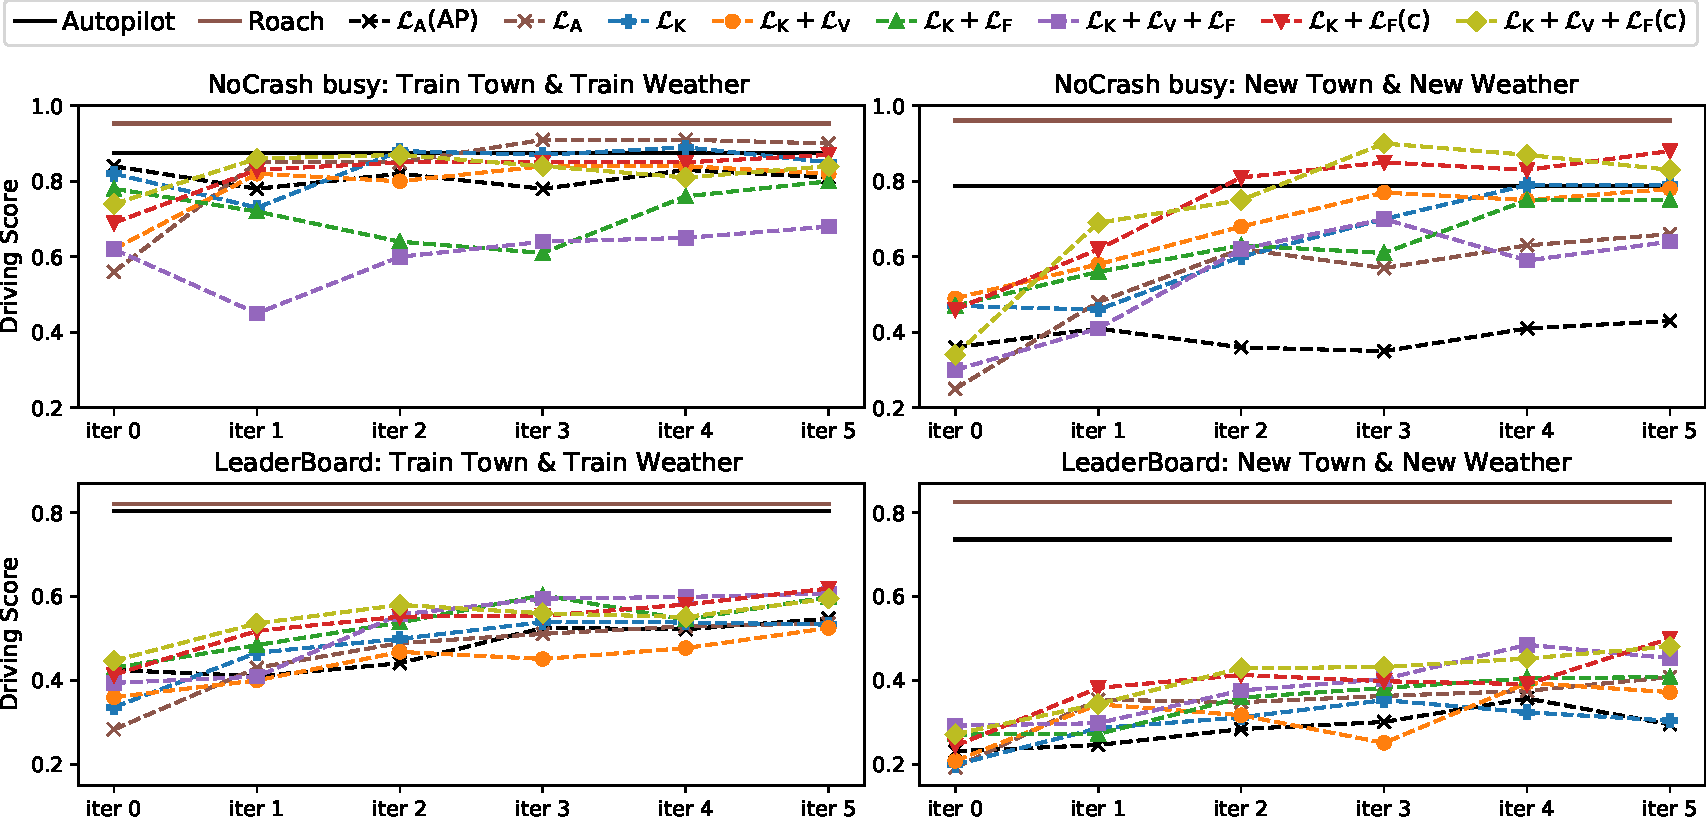
\includegraphics[width=0.99\textwidth]{img/score_eu_lb_tt_tn.pdf}
	\vspace{-1ex}
	\caption{\textbf{Driving score of experts and IL agents.} All IL agents (dashed lines) are supervised by Roach except for $\mathcal{L}_\text{A}(\text{AP})$, which is supervised by our Autopilot. For IL agents at the 5th iteration on NoCrash and all experts, results are reported as the mean over 3 evaluation seeds. Others are evaluated with one seed. The offline Leaderboard benchmark is used here.}
	\vspace{-1.5ex}
	\label{fig:score_eu_lb_tt_tn}
\end{figure*}


% table:sucess_rate_nc_dense
\begin{table}
	\setlength{\tabcolsep}{2.67pt}
	\centering
	\begin{tabular}{lccccc}
		\toprule
		Success Rate \% $\uparrow$
		&  NCd-tt & NCd-tn  & NCd-nt & NCd-nn  \\ 
		\cmidrule(lr){1-1}\cmidrule(lr){2-5}
		LBC \cite{chen2020learning} (0.9.6) & 
		$71 \pm 5$ & $63 \pm 3$ & $51 \pm 3$ & $39 \pm 6$ \\
		SAM \cite{zhao2021sam} (0.8.4) & 
		$54 \pm 3$ & $47 \pm 5$ & $29 \pm 3$ & $29 \pm 2$ \\
		LSD \cite{ohn2020learning} (0.8.4) & 
		N/A & N/A & $30 \pm 4$ & $32 \pm 3$ \\
		DA-RB\textsuperscript{+}(E) \cite{prakash2020exploring} & 
		$66 \pm 5$ & $56 \pm 1$ & $36 \pm 3$ & $35 \pm 2$ \\
		DA-RB\textsuperscript{+} \cite{prakash2020exploring} (0.8.4)  & 
		$62 \pm 1$ & $60 \pm 1$ & $34 \pm 2$ & $25 \pm 1$ \\
		Our baseline, $\mathcal{L}_\text{A}\text{(AP)}$ & 
		$\mathbf{88} \pm 4$ & $29 \pm 3$ & $32 \pm 11$ & $28 \pm 4$ \\
		Our best, $\mathcal{L}_\text{K}+\mathcal{L}_\text{F}(\text{c})$ & 
		$86 \pm 5$ & $\mathbf{82} \pm 2$ & $\mathbf{78} \pm 5$ & $\mathbf{78} \pm 0$ \\
		\bottomrule
	\end{tabular}
	\vspace{-1ex}
	\caption{\textbf{Success rate of camera-based end-to-end IL agents on NoCrash-dense.} 
		Mean and standard deviation over 3 seeds. 
		Our models are from DAGGER iteration 5. 
		For DA-RB, + means triangular perturbations are added to the off-policy dataset, (E) means ensemble of all iterations.}
	\label{table:sucess_rate_nc_dense}
	\vspace{-2ex}
\end{table}

\begin{table*}
	\setlength{\tabcolsep}{3.8pt}
	\centering
	\begin{tabular}{lccccccccc} 
		\toprule
		& \begin{tabular}{@{}c@{}}Success \\ rate \end{tabular} 
		& \begin{tabular}{@{}c@{}}Driving \\ score \end{tabular} 
		& \begin{tabular}{@{}c@{}}Route \\ compl. \end{tabular} 
		& \begin{tabular}{@{}c@{}}Infrac. \\ penalty \end{tabular} 
		& \begin{tabular}{@{}c@{}}Collision \\ others \end{tabular} 
		& \begin{tabular}{@{}c@{}}Collision \\ pedestrian \end{tabular} 
		& \begin{tabular}{@{}c@{}}Collision \\ vehicle \end{tabular}  
		& \begin{tabular}{@{}c@{}}Red light \\ infraction \end{tabular}  
		& \begin{tabular}{@{}c@{}}Agent \\ blocked \end{tabular}  \\
		\cmidrule(lr){1-1}\cmidrule(lr){2-5}\cmidrule(lr){6-10}
		iter 5
		& \%, $\uparrow$
		& \%, $\uparrow$
		& \%, $\uparrow$
		& \%, $\uparrow$
		& \#/Km, $\downarrow$
		& \#/Km, $\downarrow$
		& \#/Km, $\downarrow$
		& \#/Km, $\downarrow$
		& \#/Km, $\downarrow$
		\\
		\cmidrule(lr){1-1}\cmidrule(lr){2-5}\cmidrule(lr){6-10}
		$\mathcal{L}_\mathrm{A}(\text{AP})$
		& $31 \pm 7$ & $43 \pm 2$ & $62 \pm 6$ & $77 \pm 4$ 
		& $0.54 \pm 0.53$ & $\mathbf{0}\pm0$ & $0.63 \pm 0.50$ & $3.33 \pm 0.58$ & $19.4\pm 14.4$ \\
		$\mathcal{L}_\text{A}$
		& $57\pm7$ & $66\pm3$ & $84\pm3$ & $76\pm1$ 
		& $2.07\pm1.37$ & $\mathbf{0}\pm0$ & $1.36\pm1.10$ & $1.4\pm0.2$ & $2.82\pm1.45$ \\
		$\mathcal{L}_\text{K}$
		& $74\pm3$ & $79\pm0$ & $91\pm2$ & $86\pm1$ 
		& $0.50\pm0.25$ & $\mathbf{0}\pm0$ & $0.53\pm0.18$ & $0.68\pm0.08$ & $3.39\pm0.20$ \\
		$\mathcal{L}_\text{K}+\mathcal{L}_\text{F}(\text{c})$
		& $\mathbf{87} \pm 5$ & $\mathbf{88} \pm 3$ & $\mathbf{96} \pm 0$ & $\mathbf{91} \pm 3$ 
		& $\mathbf{0.08} \pm 0.04$ & $0.01 \pm 0.02$ & $\mathbf{0.23} \pm 0.08$ & $\mathbf{0.61} \pm 0.23$ & $\mathbf{0.84} \pm 0.04$ \\
		\cmidrule(lr){1-1}\cmidrule(lr){2-5}\cmidrule(lr){6-10}
		Roach
		& $95 \pm 2$ & $96 \pm 3$ & $100 \pm 0$ & $96 \pm 3$ 
		& $0 \pm 0$ & $0.11 \pm 0.07$ & $0.04 \pm 0.05$ & $0.16 \pm 0.20$ & $0 \pm 0$ \\
		Autopilot
		& $91 \pm 1$ & $79 \pm 2$ & $98 \pm 1$ & $80 \pm 2$ 
		& $0 \pm 0$ & $0 \pm 0$ & $0.18 \pm 0.08$ & $1.93 \pm 0.23$ & $0.18 \pm 0.08$\\
		\bottomrule
	\end{tabular}
	\vspace{-1ex}
	\caption{\textbf{Driving performance and infraction analysis of IL agents on NoCrash-busy, new town \& new weather.} 
		Mean and standard deviation over 3 evaluation seeds.}
	\vspace{-2.5ex}
	\label{table:infraction}
\end{table*}


\subsubsection{Visualizing CIL++'s Attention}
\label{sec:Visualization}
We are  interested in the image content to which CIL++ pays attention. 
Following Grad-CAM \cite{Selvaraju:2017}, gradients flow from the action space to the final convolutional layer of the ResNet backbone. 
This should produce a map that highlights the important image areas for action prediction. 
However, since CIL++ solves a regression task, its output could be either negative or positive values, while Grad-CAM is originally designed for image classification tasks which always provide positive outputs. 
To adapt Grad-CAM to our case, we cannot merely take into account the positive gradient of the feature map. 
The computation should be divided into two cases depending on the sign of the output value. 
Negative gradients are used to calculate the weights for the feature map when the acceleration or steering angle value is lower than zero, otherwise, the positive gradient is used.


% _results\_results\CILv2\CILv2_3cam_single_lane\Eval\Valid_gradCAM_Roach_LBCRoutes_3cam_valid\30\-1\85.jpg
Fig.~\ref{fig:attention_ped_greed} shows the activation map at an intersection. 
Three image areas are highly activated: the traffic light in the right image, the crossing pedestrians in the central one, and the lane shoulder in the left one. 
Thus, we believe that CIL++ shows a proper understanding of this scene, and a clear causality between observation and action since it decides to brake due to the pedestrians, even though the traffic light is in green and a \emph{turn-left} navigation command is given.

\begin{figure*}[ht!]
	\centering
	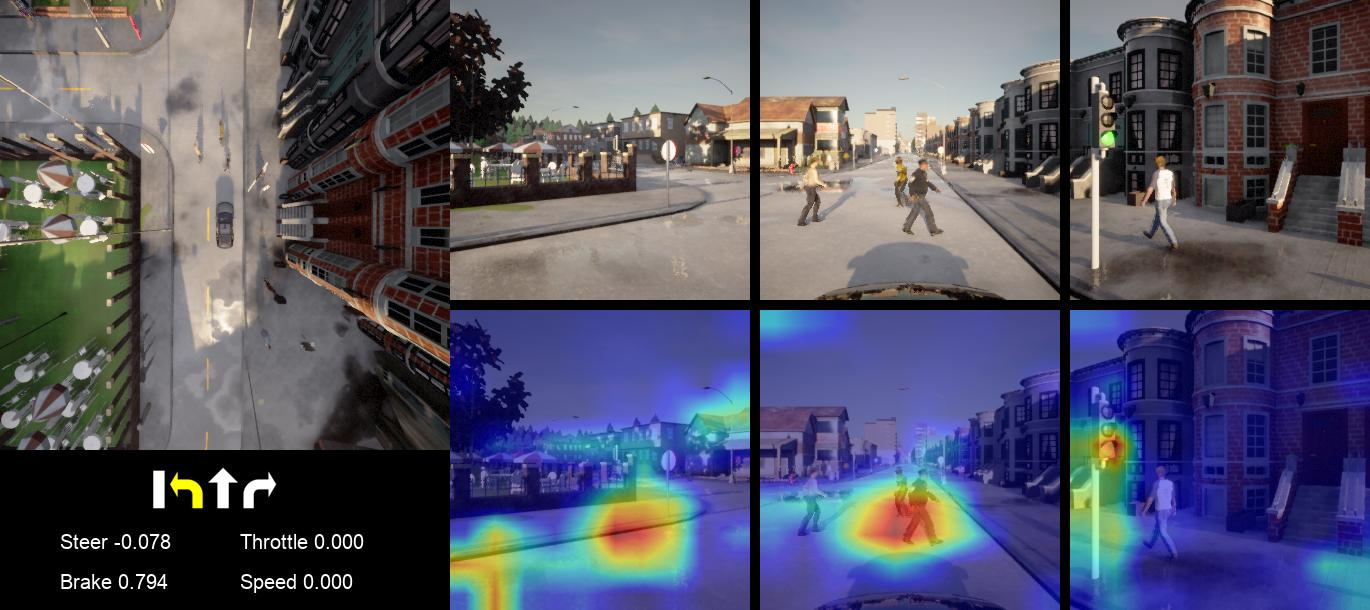
\includegraphics[width=\linewidth]{fig/attention_ped_greed.jpg}
	\caption{Activation maps of CIL++ at an intersection in Town02. 
		Three image areas from different views are highly activated: 
		the traffic light at the right image, the crossing pedestrians at the central one, and the lane shoulder at the left one. 
		Causality between observation and action is shown as a strong braking (0.794) due to the pedestrians, even though the traffic light in green and the \emph{turn-left} command.}
	\label{fig:attention_ped_greed}
\end{figure*}



\subsubsection{Ablation}

Fig.~\ref{fig:score_eu_lb_tt_tn} shows driving scores of experts and IL agents at each DAGGER iteration on NoCrash and offline LeaderBoard with busy traffic.
The baseline $\mathcal{L}_\text{A}(\text{AP})$ is our implementation of DA-RB\textsuperscript{+} supervised by our Autopilot. 
Given our improved Autopilot, it is expected that $\mathcal{L}_\text{A}(\text{AP})$ can achieve higher success rates than those reported in the DA-RB paper, but this is not observed in Table~\ref{table:sucess_rate_nc_dense}.
The large performance gap between the Autopilot and $\mathcal{L}_\text{A}(\text{AP})$ (cf. Fig.~\ref{fig:score_eu_lb_tt_tn}), especially while generalizing to a new town and new weather, indicates the limitation of this baseline.


By replacing the Autopilot with Roach, $\mathcal{L}_\text{A}$ performs better overall than $\mathcal{L}_\text{A}(\text{AP})$.
Further learning from the action distribution, $\mathcal{L}_\text{K}$ generalizes better than $\mathcal{L}_\text{A}$ on the NoCrash but not on the offline LeaderBoard.
Feature matching only helps when $\mathbf{j}_\text{IL}$ is provided with the necessary information needed to reproduce $\mathbf{j}_\text{RL}$.
In our case, $\mathbf{j}_\text{RL}$ contains navigational information as the desired route is rendered in the BEV input.
For the LeaderBoard, navigational information is partially encoded in $\mathbf{m}_\text{IL}$, which includes the vector to the next desired waypoint, so better performance is observed by using $\mathcal{L}_\text{F}$.
But for NoCrash this information is missing as $\mathbf{m}_\text{IL}$ is just the speed, hence it is impractical for $\mathbf{j}_\text{IL}$ to mimic $\mathbf{j}_\text{RL}$ and this causes the inferior performance of $\mathcal{L}_\text{K}+\mathcal{L}_\text{F}$ and $\mathcal{L}_\text{K}+\mathcal{L}_\text{F}+\mathcal{L}_\text{V}$.
To confirm this hypothesis, we evaluate a single-branch network architecture where the measurement vector $\mathbf{m}_\text{IL}$ is augmented by the command encoded as a one-hot vector.
Using feature matching with this architecture, $\mathcal{L}_\text{K}+\mathcal{L}_\text{F}(\text{c})$ and $\mathcal{L}_\text{K}+\mathcal{L}_\text{V}+\mathcal{L}_\text{F}(\text{c})$ achieve the best driving score among IL agents in the NoCrash new town \& weather generalization test, even outperforming the Autopilot.


Using value supervision in addition to feature matching helps the DAGGER process to converge faster as shown by $\mathcal{L}_\text{K}+\mathcal{L}_\text{V}+\mathcal{L}_\text{F}$ and $\mathcal{L}_\text{K}+\mathcal{L}_\text{V}+\mathcal{L}_\text{F}(\text{c})$.
However, without feature matching, using value supervision alone $\mathcal{L}_\text{K}+\mathcal{L}_\text{V}$ does not demonstrate superior performance.
This indicates a potential synergy between feature matching and value estimation.
Intuitively, the latent feature of Roach encodes the information needed for value estimation, hence mimicking this feature should help to predict the value,
while value estimation could help to regularize feature matching.


\subsubsection{Comparison with the State-of-the-art}

In Table~\ref{table:sucess_rate_nc_dense} we compare the baseline $\mathcal{L}_\text{A}(\text{AP})$ and our best performing agent $\mathcal{L}_\text{K}+\mathcal{L}_\text{F}(\text{c})$ with the state-of-the-art on the NoCrash-dense benchmark.
Our $\mathcal{L}_\text{A}(\text{AP})$ performs comparably to DA-RB\textsuperscript{+} except when generalizing to the new weather, where there is an incorrect rendering of after-rain puddles on CARLA 0.9.11 (see supplement for visualizations).
This issue does not affect our best method $\mathcal{L}_\text{K}+\mathcal{L}_\text{F}(\text{c})$ due to the stronger supervision of Roach. 
By mimicking the weather-agnostic Roach, the performance of our IL agent drops by less than $10\%$ while generalizing to the new town and weather.
Hence if the Autopilot is considered the performance upper-bound, it is fair to claim our approach saturates the NoCrash benchmark.
However, as shown in Fig.~\ref{fig:score_eu_lb_tt_tn}, there is still space for improvement on NoCrash compared to Roach and the performance gap on the offline LeaderBoard highlights the importance of this new benchmark.


\subsubsection{Performance and Infraction Analysis}

Table~\ref{table:infraction} provides the detailed performance and infraction analysis on the NoCrash benchmark with busy traffic in the new town \& weather setting.
Most notably, the extremely high ``Agent blocked'' of our baseline $\mathcal{L}_\text{A}(\text{AP})$ is due to reflections from after-rain puddles.
This problem is largely alleviated by imitating Roach, which drives more naturally, and $\mathcal{L}_\text{A}$ shows an absolute improvement of $23\%$ in terms of driving score.
In other words this is the gain achieved by using a better expert, but the same imitation learning approach. 
Further using the improved supervision from soft targets and latent features results in our best model $\mathcal{L}_\text{K}+\mathcal{L}_\text{F}(\text{c})$, which demonstrates another $22\%$ absolute improvement.
By handling red lights in a better way, this agent achieves $88\%$, an expert-level driving score, using a single camera image as input.



 